\chapter{Detailed architecture of G-EOT}
    \label{app:detailed_architecture}
    
The following two figures were generated using the tensorflow.keras.utils.plot\_model method.

\begin{figure}[h]
    \centering
    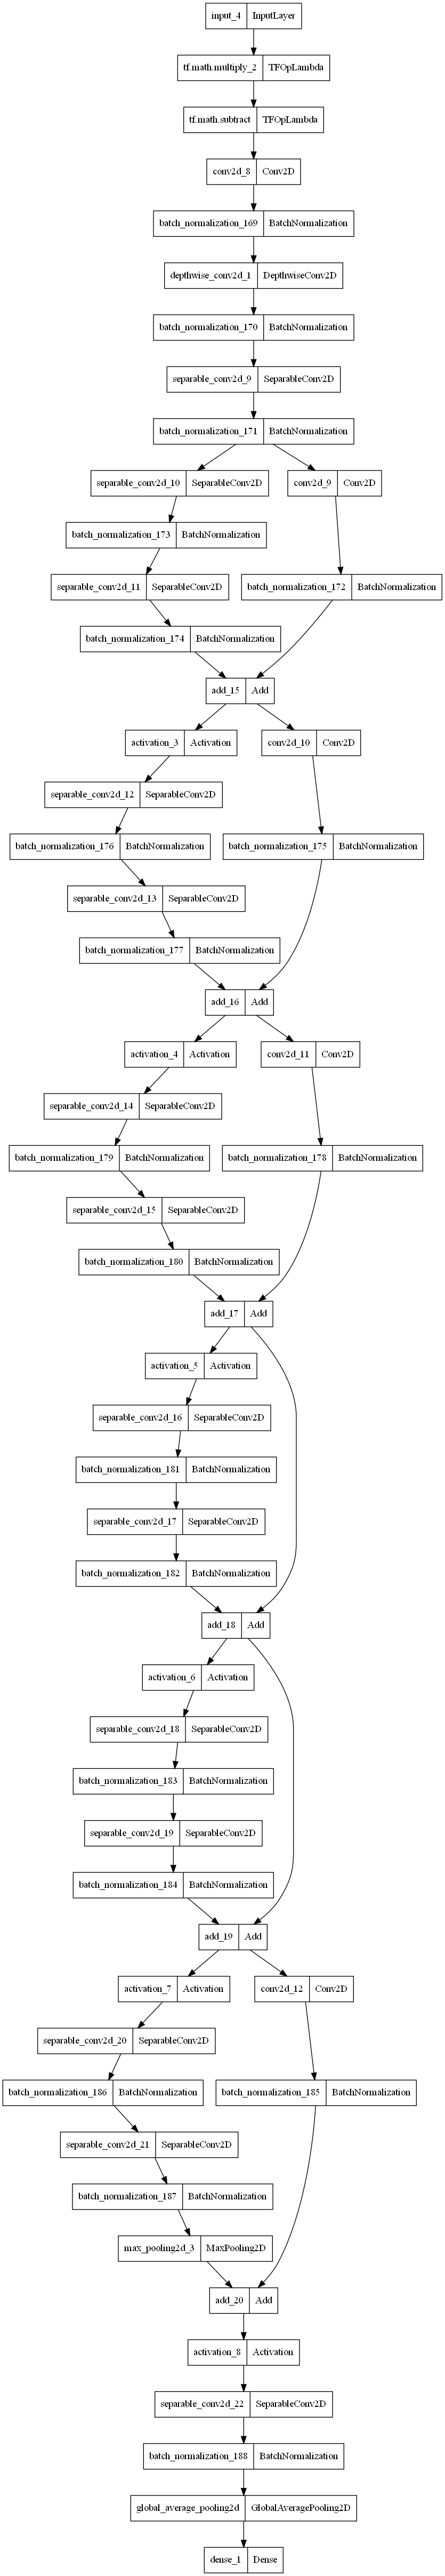
\includegraphics[width=0.24\textwidth]{graphics/detailed_simulator.png}
    \caption{Detailed diagram of the simulator of G-EOT.}
\end{figure}

\begin{figure}[h]
    \centering
    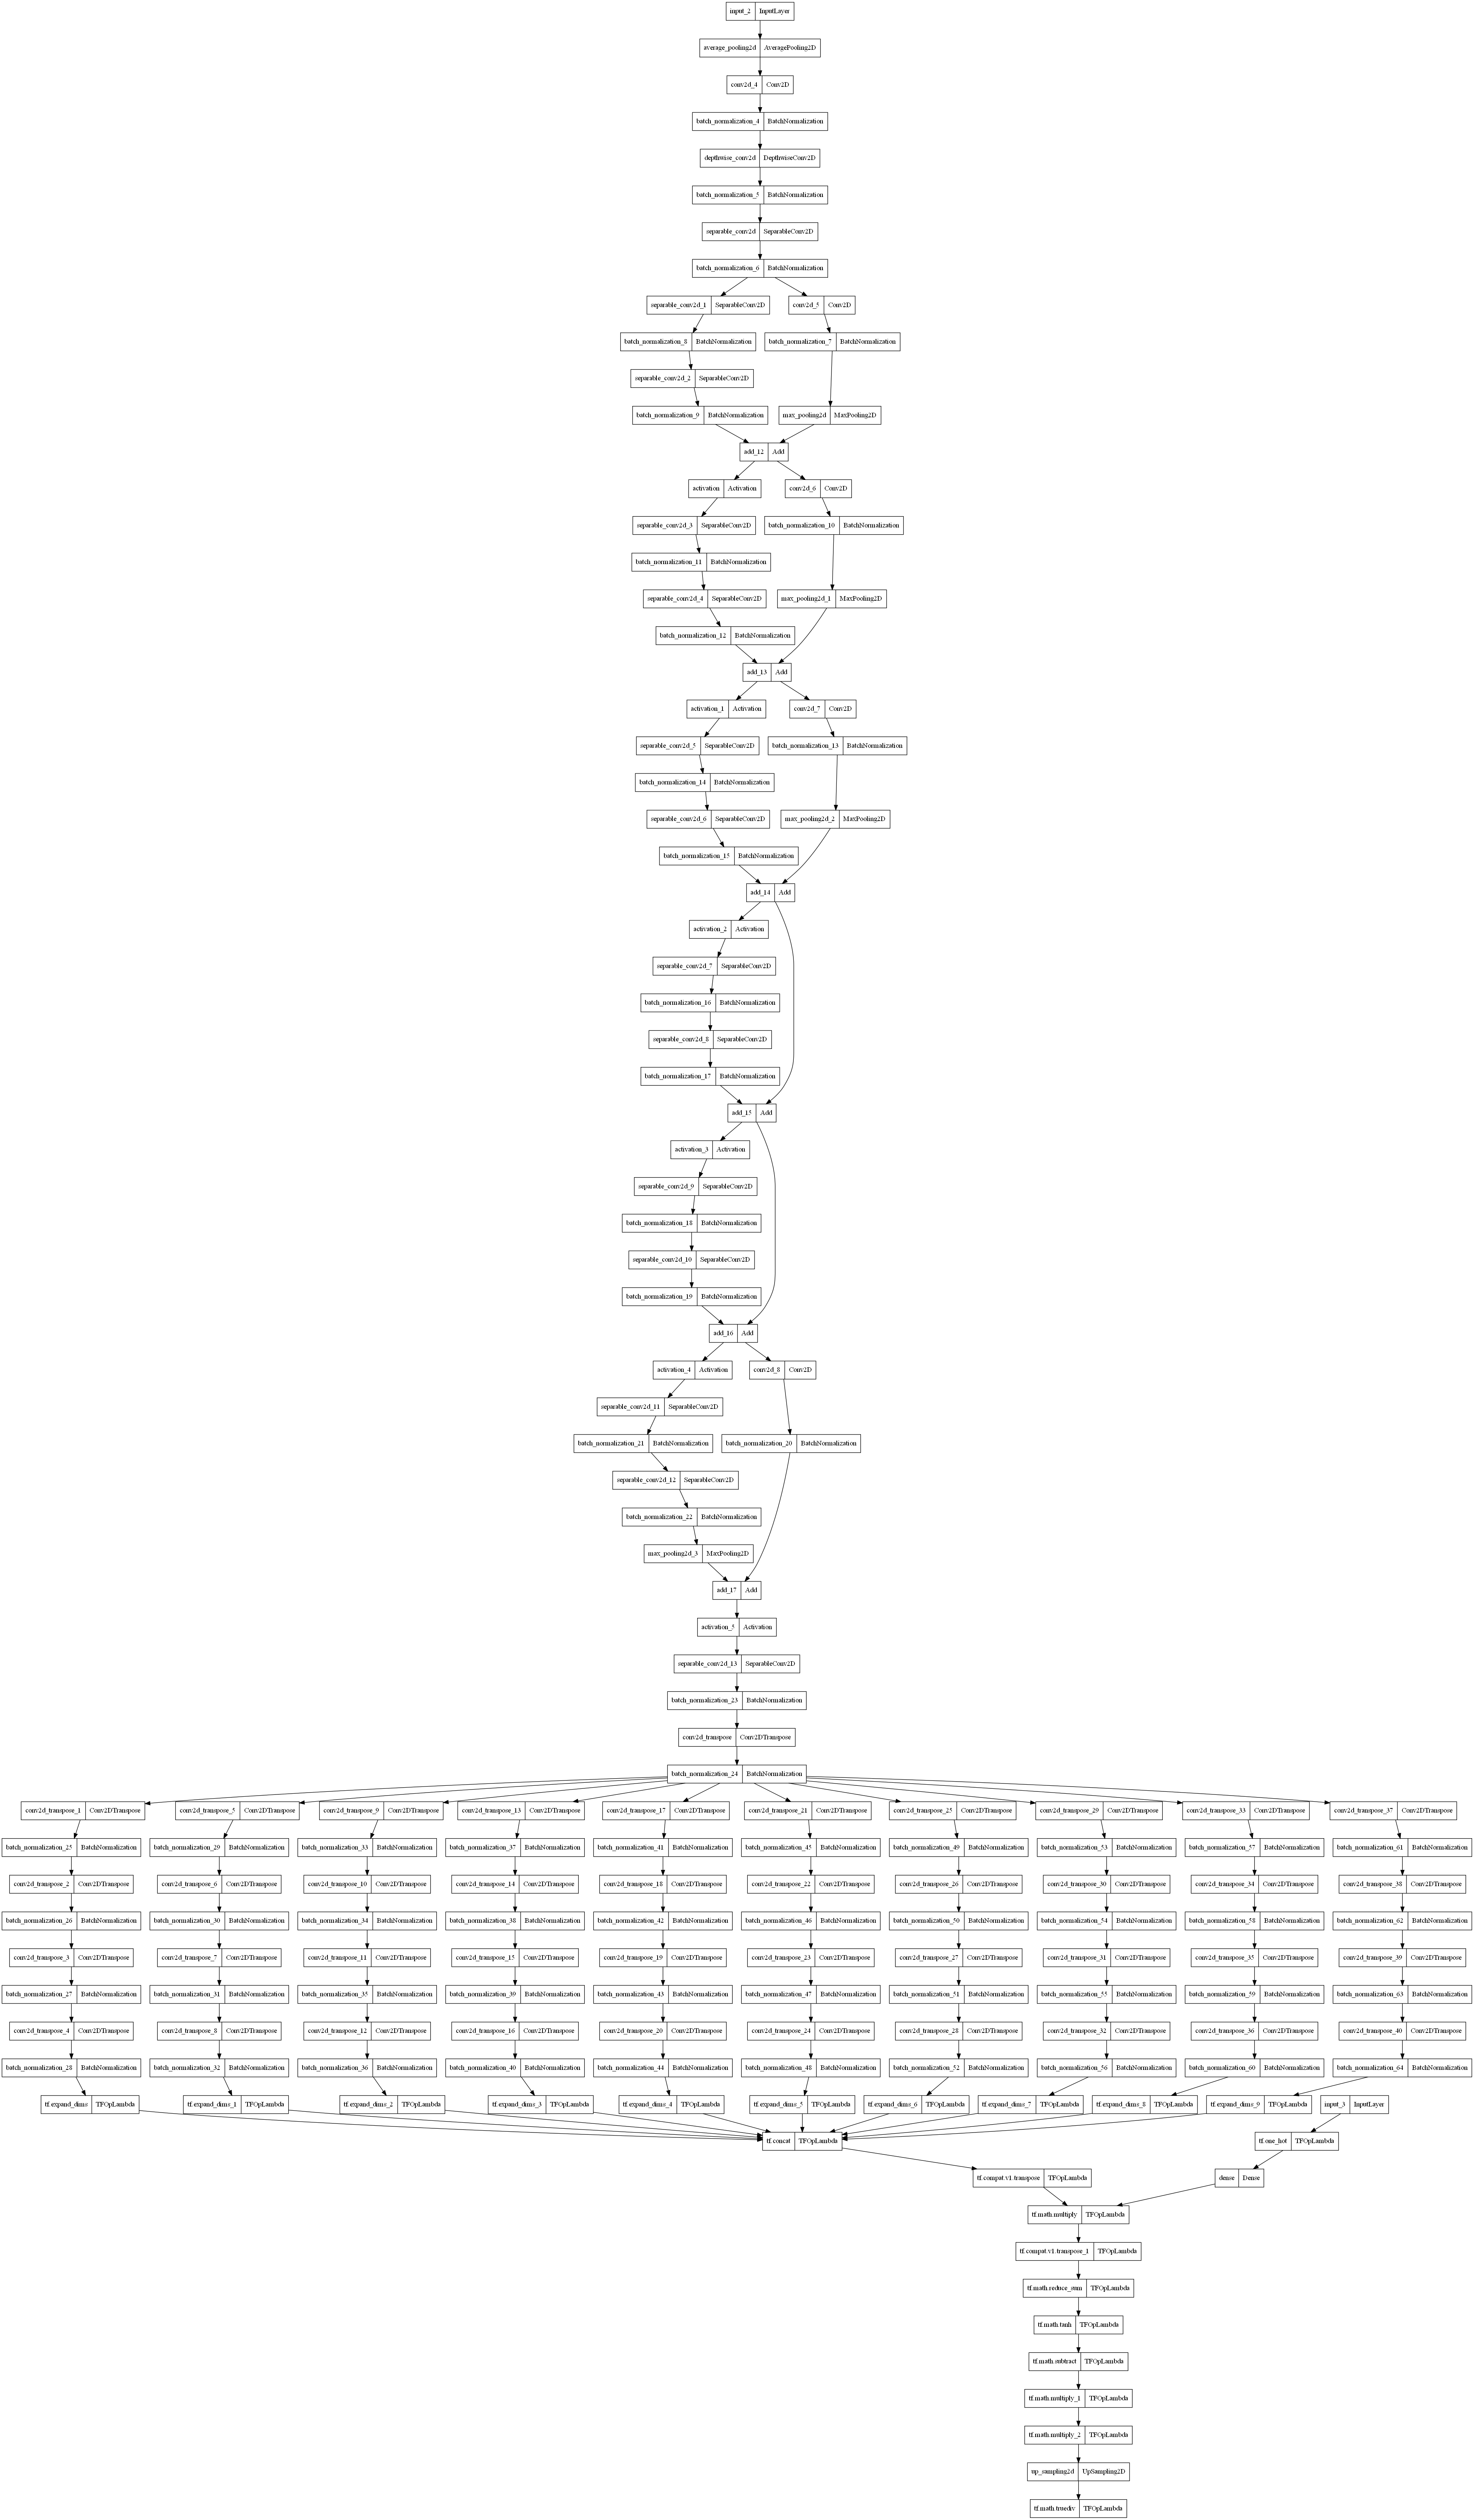
\includegraphics[width=0.8\textwidth]{graphics/detailed_generator.png}
    \caption[Detailed diagram of the generator of G-EOT.]{Detailed diagram of the generator of G-EOT. This is the version with just 10 experts, as a picture with 50 experts would have been too wide to include in this document.}
\end{figure}

\chapter{Credits for 3D models}
    \label{app:model_credits}

\begin{table}
\caption{Web links from where each 3D model in the dataset was downloaded.}
\begin{tabular}{|p{1.5cm} | p{12.5cm}|} 
 \hline
 Name & URL \\ [0.5ex] 
 \hline
 \hline
 barrel & https://free3d.com/3d-model/barrel-7685.html \\ 
 \hline
 baseball & https://www.cgtrader.com/free-3d-models/sports/equipment/game-ready-worn-baseball-ball \\ [1ex] 
 \hline
 camaro & https://free3d.com/3d-model/chevrolet-camaro-46813.html \\
 \hline
 crocodile & https://free3d.com/3d-model/crocodile-v1--688517.html \\
 \hline
 clownfish & https://sketchfab.com/3d-models/clownfish-47ba2679d91a4f14b3fc0bf8e3805af5 \\
 \hline
 crocodile & https://free3d.com/3d-model/crocodile-v1--688517.html \\
 \hline
 german shepherd & https://www.cgtrader.com/free-3d-models/animals/other/german-shepherd-dog-203601c4-4783-40e5-ab32-afa14e042dd5 \\
 \hline
 jeep & https://www.cgtrader.com/free-3d-models/car/suv/uaz-3d \\
 \hline
 orange & https://free3d.com/3d-model/-orange--470103.html \\
 \hline
 orca & https://www.cgtrader.com/items/3331128/download-page \\
 \hline
 purse & https://www.cgtrader.com/free-3d-models/household/other/small-bag-wallet \\
 \hline
 rugby ball & https://free3d.com/3d-model/rugby-ball-v1--585369.html \\
 \hline
 running shoe & https://app.gazebosim.org/GoogleResearch/fuel/models/ASICS\_GELBlur33\_20 \_GS\_BlackWhiteSafety\_Orange \\
 \hline
 turtle & https://free3d.com/3d-model/sea-turtle-v1--175922.html \\
 \hline
 taxi & https://free3d.com/3d-model/taxi-v2--375169.html \\
 \hline
 teddy & https://free3d.com/3d-model/teddy-bear-sg-v1--215992.html \\
 \hline
\end{tabular}
\end{table}

\chapter{Links to Jupyter notebooks, adversarial textures and evaluation images}
    \label{app:adversarial_textures}
    
The Jupyter Notebook used to evaluate the 50 adversarial textures created by EOT, with the full results, can be found at https://github.com/Alexandru-Dascalu/adversarial-3d/blob/master/evaluation.ipynb . It includes the TFR and classification accuracy for each adversarial texture. 

The rendered images of the adversarial 3D objects used to evaluate the adversarial textures, created by the above Jupyter notebook, can be found at https://drive.google.com/drive/folders/1IndIDIvWwXQ2mo1EXpx2LLf8m0QEfJwS?usp=sharing . The "adv" folder contains the images with the adversarial texture, while the "normal" folder has the equivalent images with the original texture. Inside both of those folders, there is a folder for each 3D model. Inside each of those folders, the photos are organised into 5 sub-folders, one for each target label.

The Jupyter notebook used to create the 50 adversarial textures and which contains the plots of the loss and TFR history during the optimisation process can be found at https://github.com/Alexandru-Dascalu/adversarial-3d/blob/master/experiments.ipynb .

The 50 adversarial textures created in the experiment in section \ref{sec:eot_experiment} can be found at https://drive.google.com/drive/folders/16zr4nH81PVdYs231k5-qpgMP1Eg6-H2x?usp=sharing . In the file name of each texture, the first number if the target label for which that texture was made, and the second number is the number of optimisation steps that took to create that texture.

The training history of the version of G-EOT with 50 experts can be seen in the Jupyter notebook at https://github.com/Alexandru-Dascalu/G-EOT/blob/master/experiment.ipynb .


